\documentclass[12pt, a4paper]{article}

% Preamble
\usepackage{xeCJK}
\usepackage[utf8]{inputenc}
\usepackage[english]{babel}
\usepackage[margin=1in]{geometry}
\usepackage[parfill]{parskip}
\usepackage{listings}
\usepackage{graphics}
\usepackage{graphicx}
\usepackage{nasm/lang}
\usepackage{nasm/style}
\usepackage{c/style}
\usepackage{go/lang}
\usepackage{go/style}
\usepackage{reil/lang}
\usepackage{llvm/lang}
\usepackage{diff/lang}
\usepackage{diff/style}
\usepackage{dot/lang}
\usepackage{dot/style}
\usepackage{float}
\usepackage[colorlinks,linkcolor=blue]{hyperref}


% Document

\usepackage{etoolbox}
\makeatletter
\def\@xobeysp{\hspace{0pt}\mbox{ }\hspace{0pt}}
\appto\verbatim@font{\hyphenchar\font`-\relax}
\apptocmd\@sverb{\hspace*{0pt}}{}{}
\makeatother

\title{COD\_LAB1 运算器的实现}
\author{黄业琦 PB17000144}
\date{March 22, 2019}
\begin{document}
\maketitle
\definecolor{vgreen}{RGB}{104,180,104}
\definecolor{vblue}{RGB}{49,49,255}
\definecolor{vorange}{RGB}{255,143,102}
\lstdefinestyle{verilog-style}
{
	language=Verilog,
	basicstyle=\small\ttfamily,
	keywordstyle=\color{vblue},
	identifierstyle=\color{black},
	commentstyle=\color{vgreen},
	numbers=left,
	numberstyle=\tiny\color{black},
	numbersep=7pt,
	tabsize=4,
	literate=*{:}{{\textcolor{black}{:}}}1
}
\section{实验目的}
\subsection{实现运算器}
Verilog实现算术逻辑单元ALU\\
s:功能选择。加、减、与、或、非、异或等运算\\
a, b:两操作数。对于减运算,a是被减数;对于非运算,操作数是a\\
y:运算结果。和、差 …… \\
f:标志。进位/借位、溢出、零标志\\
\begin{figure}[H]
	\centering
	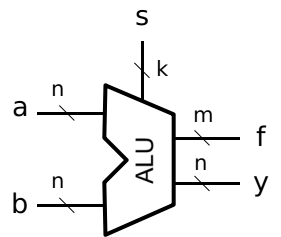
\includegraphics[width=0.4\linewidth]{ALUpic}
	\caption{ALU}
	\label{fig:alupic}
\end{figure}
\subsection{Fibonacci数列}
求给定两个初始数的斐波拉契数列(结果从同一端口分时输出)。
\subsection{求多个数的累加和}
求多个数的累加和(来自同一端口分时输入)。


\section{实验环境}
Linux下编程调试和仿真,使用IVerilog,GtkWave系列工具。\\
Windows下用于生成比特流文件,使用Vivado 2018.2,Verilog HDL\\
所有下载均在Nexsy4-DDR实验板完成

\section{逻辑设计}
\subsection{ALU设计}
目前ALU只实现了6个功能:4个逻辑运算和2个算术运算。\\
对于逻辑运算,不可能产生进位、溢出等问题。\\
算术运算考虑方法为:溢出位为直接加考虑,进位/借位考虑需要用异或实现,详细见附录代码。
\subsection{Fibonacci设计和累计求和}
我们需要额外多加register用于保存中间结果(老师毙掉了我想使用$inout$接口$+$外设输入的想法,但最后一周我还是会这么玩的)\\

\section{仿真截图}
\begin{figure}[H]
	\centering
	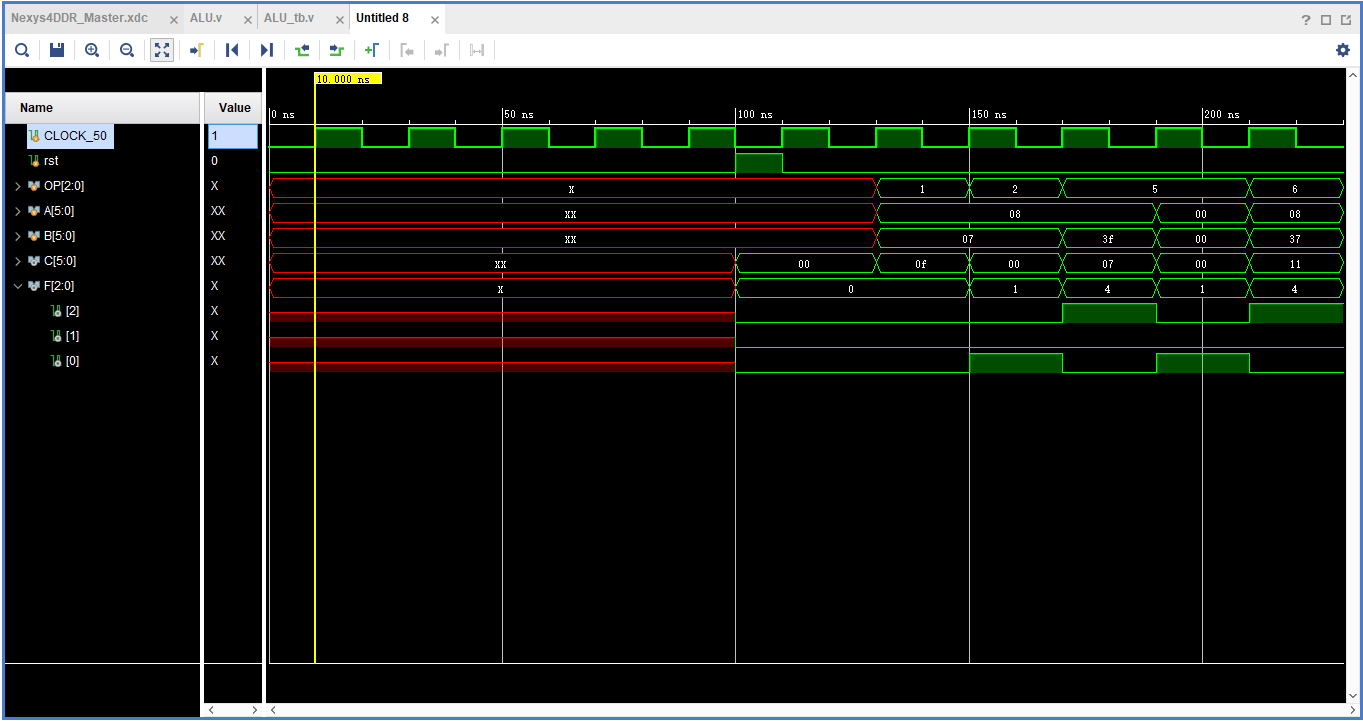
\includegraphics[width=1.0\linewidth]{VIVADO/LAB1/lab1_alu_sim}
	\caption{ALU\_sim}
	\label{fig:lab1alusim}
\end{figure}
\begin{figure}[H]
\centering
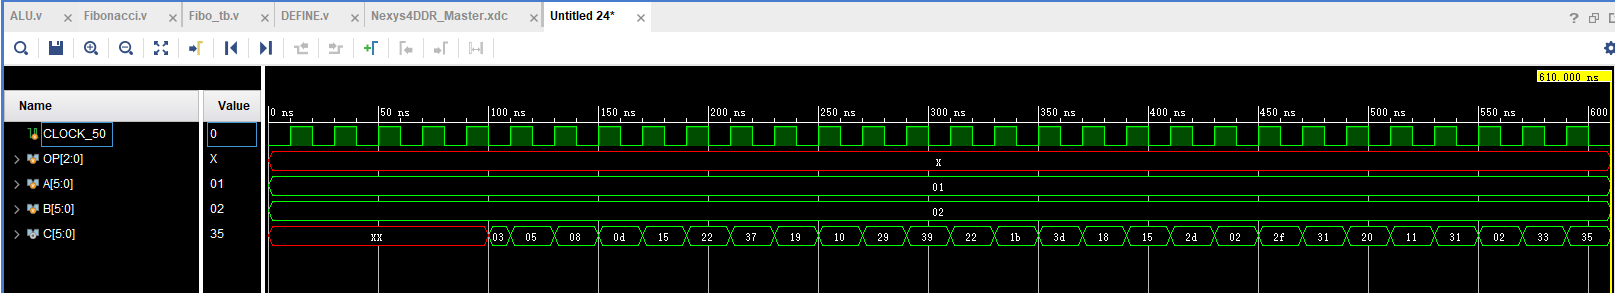
\includegraphics[width=1.0\linewidth]{/home/chivier_humber/Documents/Study/COD_LAB/LAB1/VIVADO/LAB1/Fibonacci_sim.PNG}
\caption{Fibonacci\_sim}
\label{fig:lab1alusim}
\end{figure}
\begin{figure}[H]
	\centering
	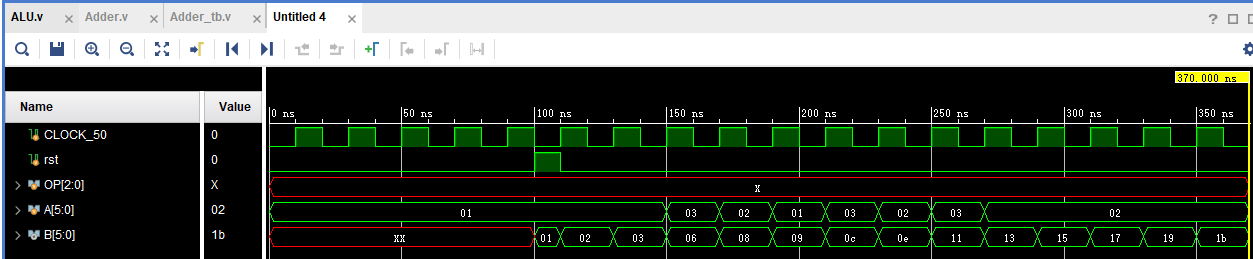
\includegraphics[width=1.0\linewidth]{/home/chivier_humber/Documents/Study/COD_LAB/LAB1/LAB1_VIVADO/Adder_sim.PNG}
	\caption{Adder\_sim}
	\label{fig:lab1alusim}
\end{figure}

\section{性能评测截图}
\begin{figure}[H]
	\centering
	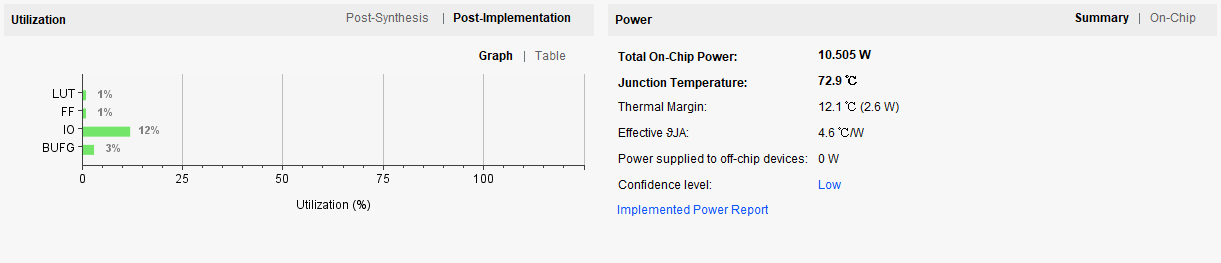
\includegraphics[width=1.0\linewidth]{/home/chivier_humber/Documents/Study/COD_LAB/LAB1/LAB1_VIVADO/ALU_Perfoemance1.PNG}
	\caption{ALU\_Perfoemance1}
	\label{fig:lab1alusim}
\end{figure}
\begin{figure}[H]
	\centering
	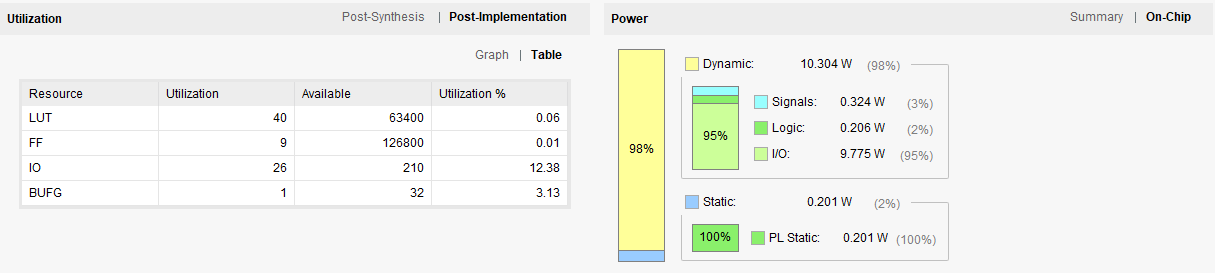
\includegraphics[width=1.0\linewidth]{/home/chivier_humber/Documents/Study/COD_LAB/LAB1/LAB1_VIVADO/ALU_Perfoemance2.PNG}
	\caption{Adder\_sim}
	\label{fig:lab1alusim}
\end{figure}
\begin{figure}[H]
	\centering
	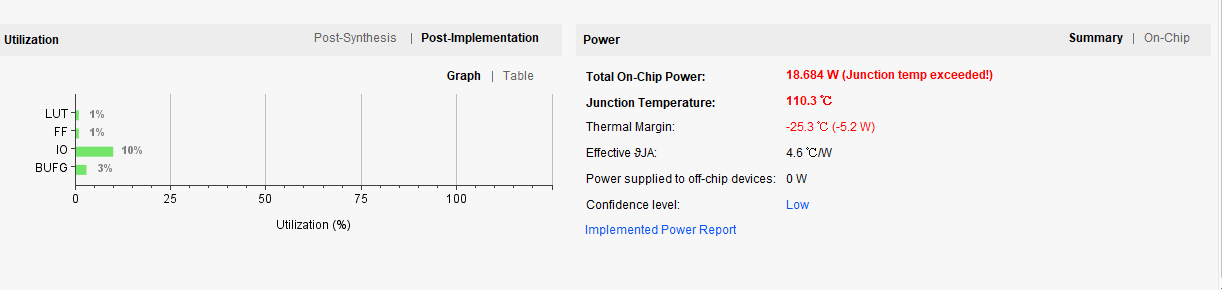
\includegraphics[width=1.0\linewidth]{/home/chivier_humber/Documents/Study/COD_LAB/LAB1/LAB1_VIVADO/Fibo_Perfoemance1.PNG}
	\caption{Fibo\_Perfoemance1}
	\label{fig:lab1alusim}
\end{figure}
\begin{figure}[H]
	\centering
	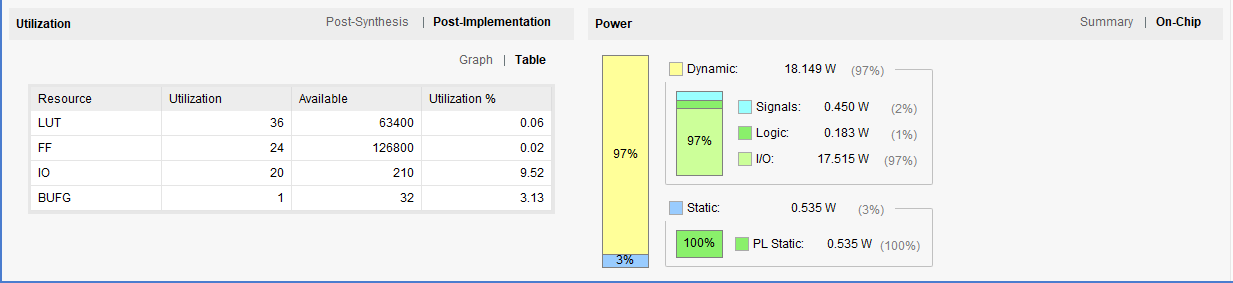
\includegraphics[width=1.0\linewidth]{/home/chivier_humber/Documents/Study/COD_LAB/LAB1/LAB1_VIVADO/Fibo_Perfoemance2.PNG}
	\caption{Fibo\_Perfoemance2}
	\label{fig:lab1alusim}
\end{figure}
\begin{figure}[H]
	\centering
	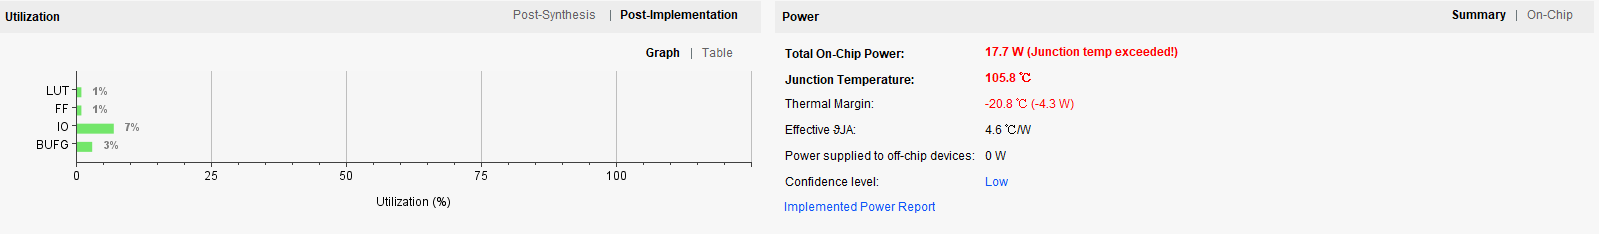
\includegraphics[width=1.0\linewidth]{/home/chivier_humber/Documents/Study/COD_LAB/LAB1/LAB1_VIVADO/Adder_Perfoemance1.PNG}
	\caption{Adder\_Perfoemance1}
	\label{fig:lab1alusim}
\end{figure}
\begin{figure}[H]
	\centering
	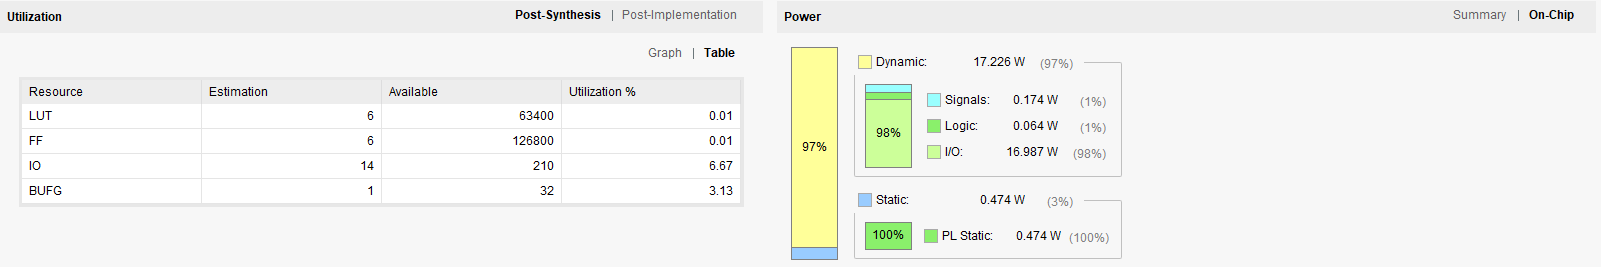
\includegraphics[width=1.0\linewidth]{/home/chivier_humber/Documents/Study/COD_LAB/LAB1/LAB1_VIVADO/Adder_Perfoemance2.PNG}
	\caption{Adder\_Perfoemance2}
	\label{fig:lab1alusim}
\end{figure}


\section{实验代码}
\subsection{ALU实现代码}
\lstinputlisting[style={verilog-style},caption={DEFINE.v}]{/home/chivier_humber/Documents/Study/COD_LAB/LAB1/CODE/ALU/DEFINE.v}
\lstinputlisting[style={verilog-style},caption={ALU.v}]{/home/chivier_humber/Documents/Study/COD_LAB/LAB1/CODE/ALU/ALU.v}
\lstinputlisting[style={verilog-style},caption={ALU\_tb.v}]{/home/chivier_humber/Documents/Study/COD_LAB/LAB1/CODE/ALU/ALU_tb.v}
\clearpage
\subsection{Fibonacci实现代码}
\lstinputlisting[style={verilog-style},caption={DEFINE.v}]{/home/chivier_humber/Documents/Study/COD_LAB/LAB1/LAB1_VIVADO/Fibonacci/DEFINE.v}
\lstinputlisting[style={verilog-style},caption={ALU.v}]{/home/chivier_humber/Documents/Study/COD_LAB/LAB1/LAB1_VIVADO/Fibonacci/ALU.v}
\lstinputlisting[style={verilog-style},caption={Fibonacci.v}]{/home/chivier_humber/Documents/Study/COD_LAB/LAB1/LAB1_VIVADO/Fibonacci/Fibonacci.srcs/sources_1/new/Fibonacci.v}
\lstinputlisting[style={verilog-style},caption={Fibo\_tb.v}]{/home/chivier_humber/Documents/Study/COD_LAB/LAB1/LAB1_VIVADO/Fibonacci/Fibonacci.srcs/sim_1/new/Fibo_tb.v}
\clearpage
\subsection{累加器实现代码}
\lstinputlisting[style={verilog-style},caption={DEFINE.v}]{/home/chivier_humber/Documents/Study/COD_LAB/LAB1/LAB1_VIVADO/Adder/DEFINE.v}
\lstinputlisting[style={verilog-style},caption={ALU.v}]{/home/chivier_humber/Documents/Study/COD_LAB/LAB1/LAB1_VIVADO/Adder/ALU.v}
\lstinputlisting[style={verilog-style},caption={Adder.v}]{/home/chivier_humber/Documents/Study/COD_LAB/LAB1/LAB1_VIVADO/Adder/Adder.srcs/sources_1/new/Adder.v}
\lstinputlisting[style={verilog-style},caption={Adder\_tb.v}]{/home/chivier_humber/Documents/Study/COD_LAB/LAB1/LAB1_VIVADO/Adder/Adder.srcs/sim_1/new/Adder_tb.v}
\clearpage

\section{实验总结}
本次试验总体算比较顺利的,中途有一处问题,再Fibonacci数列试验中,直接用了前一个实验的ALU部件,倒置clk和rst没有删去,倒置在加法时多跑了一个时间周期,出现了问题,以后需要注意。最终是重写了简单版的ALU模块替换解决了问题。
\end{document}
